\setchapterpreamble[u]{\margintoc}
\chapter{Polynômes}
\labch{polynomes}

\marginnote{Texte issu de \cite{oraux_x_ens_1}}

\begin{marginfigure}[5cm]
    \centering
    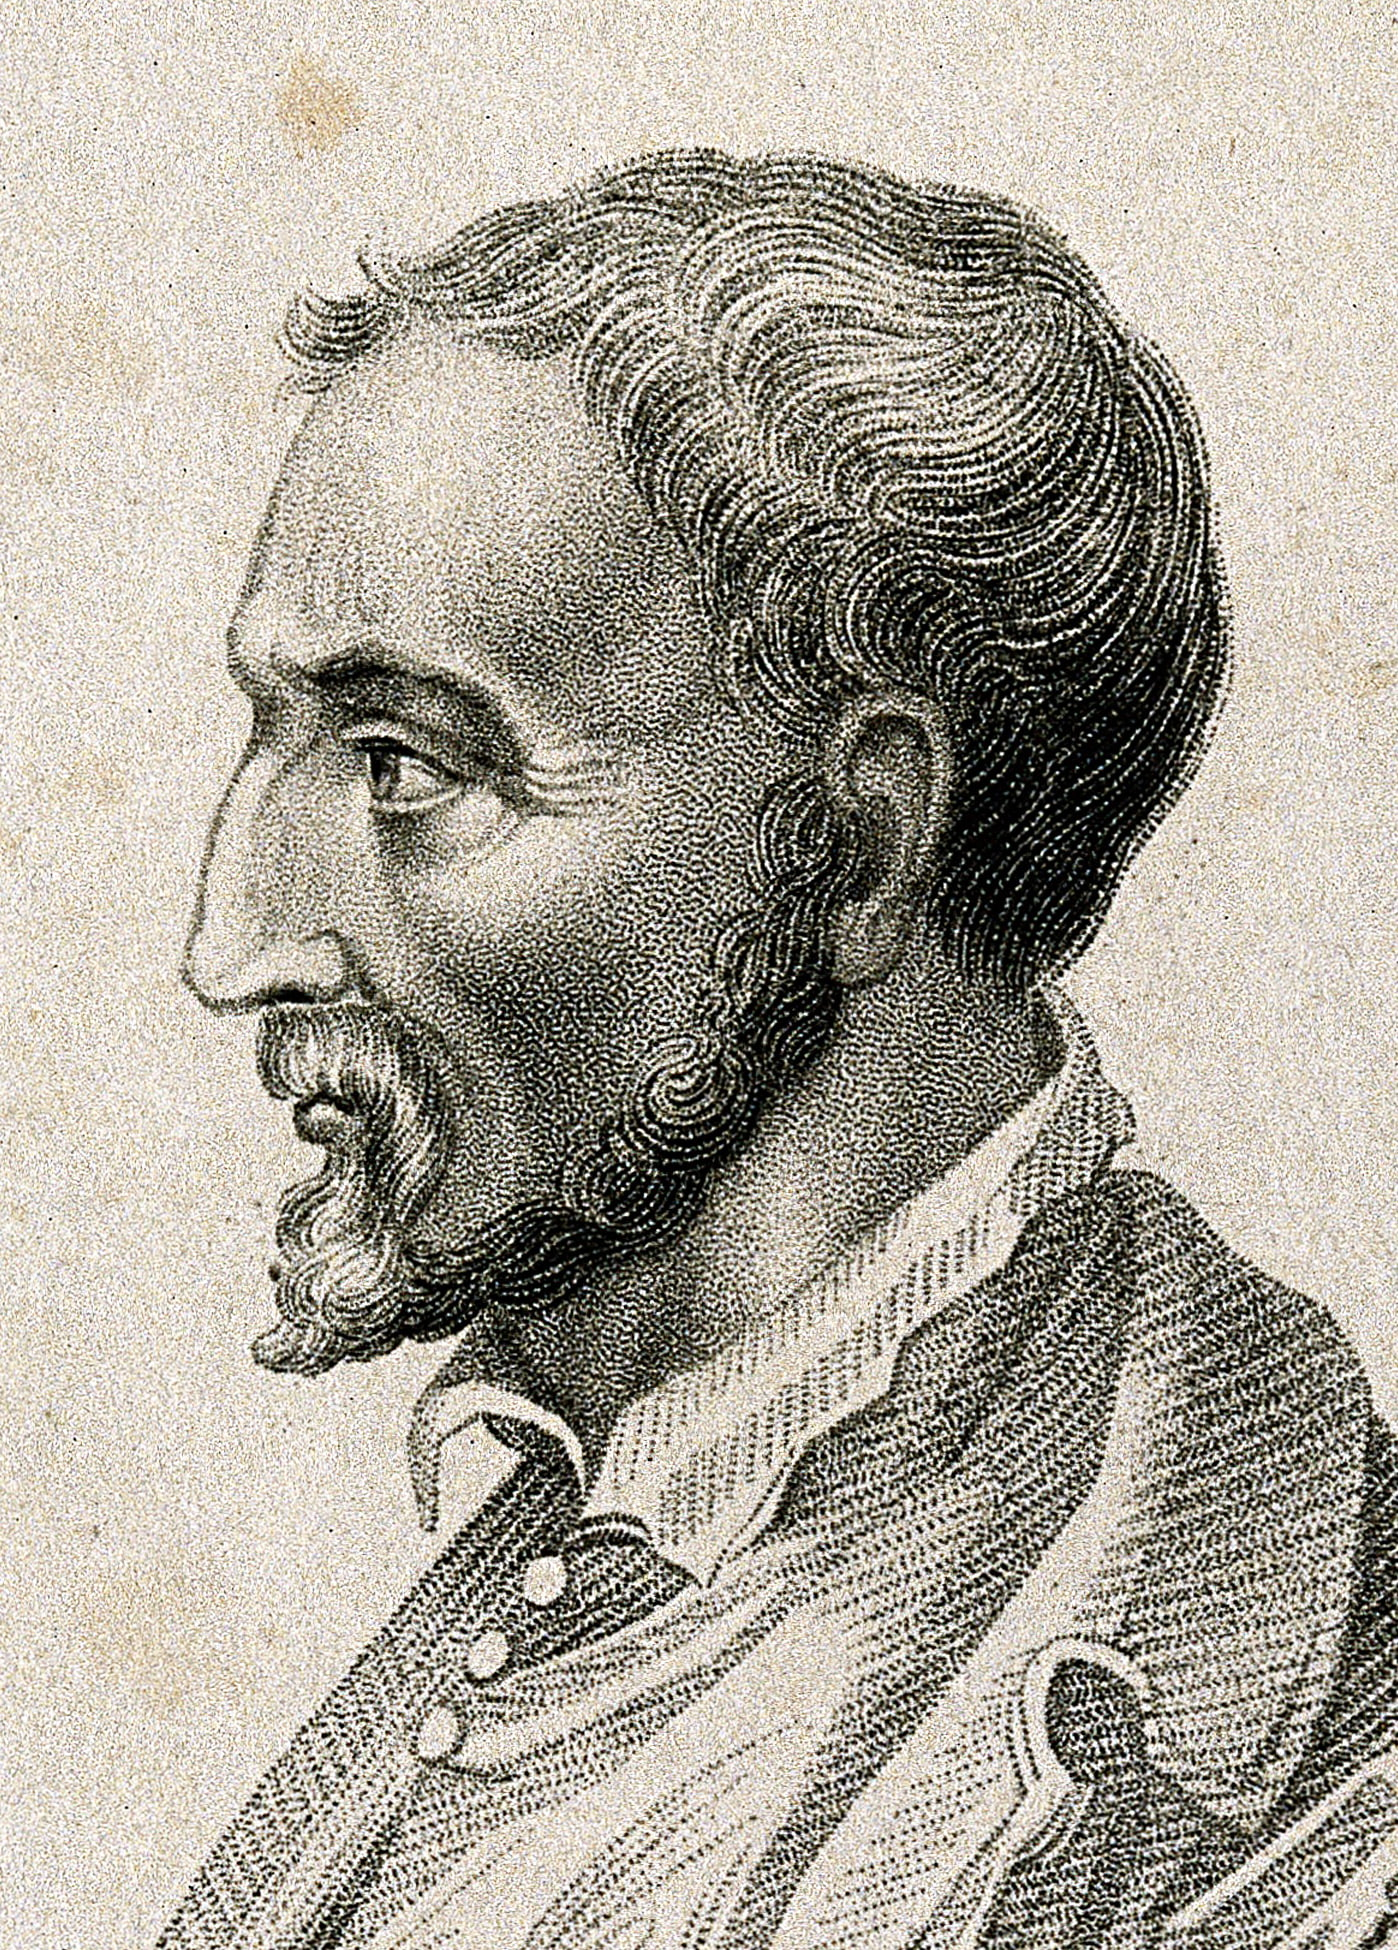
\includegraphics{images/jerome_cardan.jpg}
    \caption*{\centering Jérome \textsc{Cardan} (1501 - 1576)}
\end{marginfigure}

\textsl{
La théorie des équations polynomiales, qui précède de loin la définition formelle des polynômes, a été le propos essentiel de l'algèbre jusqu'au \textsc{xix}$^\me$ siècle. Elle est à l'origine de nombreuses notions: corps, nombres algébriques \dots Son développement est lié aux extensions successives de la notion de nombre: introduction des nombres négatifs, des nombres irrationnels, puis des nombres complexes. \\ 
Dès la plus haute Antiquité, on rencontre des exemples de résolutions d'équations. Les Babyloniens savent résoudre l'équation du second degré et les Grecs en font la base même de leur géométrie. \\
Après l'Antiquité, il faudra attendre le \textsc{xvi}$^\me$ siècle pour que des progrès substantiels apparaissent, dus à l'école italienne. \textsc{Scipone del Ferro}, \textsc{Tartaglia} et \textsc{Cardan} apportent la solution de l'équation du troisième dégré. L'équation générale est ramenée à la forme réduite $x^3 + px + q = 0$, dont une solution s'écrit
$$x = \sqrt[3]{-\frac{q}{2} + \sqrt{\frac{q^2}{4} + \frac{p^3}{27}}} + \sqrt[3]{-\frac{q}{2} - \sqrt{\frac{q^2}{4} + \frac{p^3}{27}}}.$$
Cette solution soulève des difficultés: si $\frac{q^2}{4} + \frac{p^3}{27}$ est négatif, cas où l'équation a des racines -- on le sait depuis \textsc{Archimède} -- on ne peut pas calculer $x$. Pour lever la difficulté, \textsc{Cardan} introduit timidement de nouveaux nombres, \say{ impossibles } ou \say{ imaginaires }. \textsc{Ferrari} et \textsc{Bombelli} résolvent l'équation du quatrième degré. \\
Grâce à l'école italienne, le théorie générale des équations algébriques se précise. L'équation étant mise sous le forme $P(x) = 0$, on prend conscience de l'importance du dégré de $P$ pour le nombre de solutions. On découvre que si $a$ est une racine de $P$, on peut factoriser par $x-a$. Les relations entre les coefficients et les fonctions symétriques des racines d'un polynôme apparaissent chez \textsc{Viète} (1540-1603), mais c'est \textsc{Girard} qui en 1629 leur donne toute leur extension. Suivi par \textsc{Newton}, il exprime les sommes des puissances des racines en fonction des coefficients. L'étude des fonctions symétriques des racines va se développer au \textsc{xvii}$^\me$ siècle avec \textsc{Waring} et au \textsc{xix}$^\me$ siècle avec \textsc{Cauchy}. \\
Au \textsc{xvii}$^\me$ siècle, la majorité des mathématiciens est convaincue qu'une équation de degré $n$ possède $n$ racines, celles-ci pouvant ne pas être réelles, mais il faut attendre \textsc{d'Alembert} pour trouver en 1724 une définition précise des nombres complexes (sous la forme $a + \sqrt{-1} b$). En 1799, \textsc{Gauss} fournit plusieurs preuves rigoureuses du \say{ théorème fondamental de l'algèbre } ou \say{ théorème de \textsc{d'Alembert}-\textsc{Gauss} }. \\
Des progrès sont réalisés également dans l'étude du nombre de racines réelles, et de leur signe. En 1637, \textsc{Descartes} énonce la règle qui porte son nom sur le nombre de racines positives d'un polynôme. On trouve dans \text{l'Algèbre} de \textsc{Rolle} (1690), la propriété suivante: entre deux solutions de l'équation $P(x)=0$, il existe au moins une solution de l'équation $P'(x)=0$. C'est \textsc{Sturm} qui formule, en 1829, les résultats les plus précis sur le nombre de racines réelles d'un polynôme. \\
Après les succès le l'école italienne au \textsc{xvi}$^\me$ siècle, les mathématiciens se sont attachés à trouver des formules analogues pour les dégrés suivants. Les réflexions sur cette question prennent un tour nouveau avec les travaux de \textsc{Lagrange} (1771), qui étudie les permutations des racines d'une équation laissant invariantes certaines fonctions de ces racines. Ces idées sont approfondies par \textsc{Cauchy} et \textsc{Ruffini}. \textsc{Abel} donne une démonstration rigoureuse de l'impossibilité de résoudre par radicaux l'équation générale de dégré $5$ en 1829. Enfin, en introduisant la notion de groupe, \textsc{Galois} énonce la condition générale à laquelle satisfait toute équation résoluble par radicaux (1831). \\
La distinction entre les nombres algébriques, racines d'un polynôme à coefficients entiers, et les autres qu'on nomme transcendants, date du \textsc{xvii}$^\me$ siècle, mais il faut attendre 1844 pour que \textsc{Liouville} démontre l'existence de nombres transcendants et plus longtemps encore pour que soit démontrée le trascendance de $\me$ (par \textsc{Hermite} en 1872) et celle de $\pi$ (par \textsc{Lindemann} en 1882). \\
Quant à la définition formelle des polynômes et à l'étude de leur structure, elles chemineront tout au long du \textsc{xix}$^\me$ siècle au rythme lent du processus d'axiomatisation de l'algèbre: par exemple, \textsc{Dedekind} introduit la notion de corps et définit les idéaux vers 1870.
}

\newpage

\section{Polynômes de \textsc{Legendre}} \labsec{polynomes_de_legendre}
\begin{tcolorbox}
    Pour tout $n \in \Ne$, on définit le polynôme $\Leg_n$ par:
    $$\Leg_n(X) = \frac{1}{2^n} \sum_{k=0}^{n} \binom{n}{k}^2 (X-1)^{n-k}(X+1)^{k},$$
    $$\Leg_n(X) = \frac{1}{2^n n!} \left( (X^2-1)^n \right)^{(n)}.$$
\end{tcolorbox}

Les polynômes de \textsc{Legendre} constituent l'exemple le plus simple d'une suite de polynômes orthogonaux. \\
La suite vient de \url{https://bibmath.net/dico/index.php?action=affiche&quoi=./l/legendrepoly.html}.
Les polynômes de \textsc{Legendre} sont orthogonaux pour le produit scalaire
$$\langle P, Q \rangle = \int_{-1}^1 P(t) Q(t) \d t$$
mais ne sont toutefois par orthonormaux car
$$\langle \Leg_n, \Leg_n \rangle = \frac{2}{2n+1}.$$

\begin{elem_sol}
    Pour montrer que $\Leg_n(X)$ est scindé à racines simples dans $]-1, 1[$, raisonner par récurrence et penser à \textsc{Rolle}. 
\end{elem_sol}

\begin{marginfigure}[-6cm]
	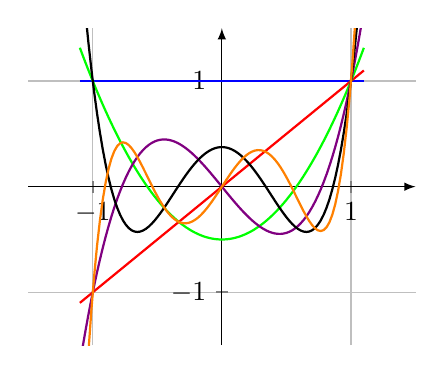
\begin{tikzpicture}
    \begin{axis}[width=6.5cm,
        axis lines=middle,
        inner axis line style={-latex},
        grid=major,
        xmin=-1.5, xmax=1.5,
        ymin=-1.5, ymax=1.5,
        % xlabel=$x$, xlabel style={right},
        % ylabel=$y$, ylabel style={above},
        tick style={thick},
        ticklabel style={font=\normalsize},
        xtick={-1, 0, 1}, 
        ytick={-1, 0, 1},
        % legend entries={0.5x},
            legend style={
            at={(1.05,0.4)},
            anchor=north,
            legend columns=1},
            legend cell align={left}
    ]
    
    \def\a{-1.1}
    \def\b{1.1}
    
    \addplot[blue,thick,samples=100,domain=\a:\b] {1};
    \addplot[red,thick,samples=100,domain=\a:\b] {x};
    \addplot[green,thick,samples=100,domain=\a:\b] {1/2*(3*x^2-1)};
    \addplot[violet,thick,samples=100,domain=\a:\b] {1/2*(5*x^3-3*x)};
    \addplot[black,thick,samples=100,domain=\a:\b] {1/8*(35*x^4-30*x^2+3)};
    \addplot[orange,thick,samples=100,domain=\a:\b] {1/8*(63*x^5-70*x^3+15*x)};
    
   % \legend{$\Leg_0$, 
   %         $\Leg_1$,
%            $\Leg_2$,
%            $\Leg_3$,
 %           $\Leg_4$,
  %          $\Leg_5$
   %         }
    \end{axis}
\end{tikzpicture}
	\caption{Les premiers polynômes de \textsc{Legendre}}
	{\scriptsize
	\color{blue} $\Leg_0 = 1$ \\ 
	\color{red} $\Leg_1 = x$ \\
	\color{green} $\Leg_2 = \frac{1}{2}(3x^2-1)$ \\
	\color{purple} $\Leg_3 = \frac{1}{2}(5x^3-3x)$ \\
	\color{black} $\Leg_4 = \frac{1}{8}(35x^4-30x^2+3)$ \\
	\color{orange} $\Leg_5 = \frac{1}{8}(63x^5-70x^3+15x)$
	}
\end{marginfigure}



\section{Polynômes de \textsc{Hilbert}} \labsec{polynomes_de_hilbert}
\begin{defi}{Polynômes de \textsc{Hilbert}}
    On appelle famille des \emph{polynômes de \textsc{Hilbert}} la suite de polynômes $(\Hilb_n)_{n \in \N}$ définie par
    $$\Hilb_0 \defeq 1,\ \forall n \in \Ne,\ \Hilb_n \defeq \frac{X(X-1)\cdots(X-n+1)}{n!}.$$
\end{defi}

Voir aussi \nameref{polynome_hilbert} dans la partie algèbre linéaire. 

\begin{exercice}
    \marginnote[0cm]{Sources : \cite{exos_oraux} p.27, \cite{fmaalouf}}
    \begin{enumerate}
        \item Montrer que pour tout $n \in \N$, $\Hilb_n(\Z) \subset \Z$. En déduire que le produit de $n$ entiers consécutifs dans $\Z$ est divisible par $n!$.
        \item Soient $n \in \Ne$ et $Q \in \R_n[X]$. Montrer que les deux assertions suivantes sont équivalentes:
        \begin{enumerate}[label=(\roman*)]
            \item $Q(\Z) \subset \Z$,
            \item $\forall m \in \llbracket 0, n \rrbracket, Q(m) \in \Z$.
            \item $\exists (\lambda_0, \dots, \lambda_n) \in \Z^{n+1} \text{ tel que } Q = \sum\limits_{k=0}^n \lambda_k \Hilb_k$.
        \end{enumerate}
    \end{enumerate}
\end{exercice}

\begin{solution}
\end{solution}

\section{Polynômes de \textsc{Bernoulli}} \labsec{polynomes_de_bernoulli}
\marginnote[0cm]{Lire \cite{calcul_infinitesimal} p. 297}
% Note d'un thème (cf. bureau) \\

Il arrive fréquemment que le calcul exact d’une intégrale soit difficile, voire
impossible pour certaines fonctions et il est courant, dans ce cas, de chercher à
approcher la valeur de l’intégrale en utilisant des polynômes comme les polynômes de \nom{Bernoulli} par exemple.

\begin{defi}[Polynômes de \nom{Bernoulli}]
    Les \emph{polynômes de \nom{Bernoulli}} forment l'unique suite de polynômes $(\Bern_n)_{n \in \N}$ telle que:
    \begin{align*}
        &\Bern_0 = 1, \\
        \forall n \in \N,\ &\Bern'_{n+1} = (n+1)\Bern_n, \\
        \forall n \in \Ne,\ &\int_{0}^{1} \Bern_n(x) \d x = 0.
    \end{align*}
\end{defi}

\begin{defi}[Nombres de \nom{Bernoulli}]
    Pour tout $n \geqslant 0$, on pose $\mathrm{b}_n \defeq \Bern_n(0)$. La suite de réels $(\mathrm{b}_n)_{n \in \N}$ est appelée suite des \emph{nombres de \nom{Bernoulli}}.
\end{defi}  

\begin{table}[H]
    \centering
    \begingroup
        \renewcommand{\arraystretch}{1.2}
        \begin{tabularx}{\textwidth}{ |c| *{10}{>{\centering\arraybackslash}X|}}
         \hline
         $n$ & $0$ & $1$ & $2$ & $3$ & $4$ & $5$ & $6$ & $7$ & $8$ \\ \hline
         $\mathrm{b}_n$ & $1$ & $-\frac{1}{2}$ & $\frac{1}{6}$ & $0$ & $-\frac{1}{30}$ & $0$ & $\frac{1}{42}$ & $0$ & $-\frac{1}{30}$ \\
         \hline
    \end{tabularx}
    \endgroup
    \caption{Valeurs des premiers nombres de \textsc{Bernoulli}}
\end{table}

\begin{exercice}
    \begin{questions}
        \item Déterminer le degré de $\Bern_n(X)$ pour $n \geqslant 0$. 
        \item Montrer que, pour tout $n \geqslant 2$, $\Bern_n(0) = \Bern_n(1)$.
        \item Soient $n \in \N$ et $x \in \R$. Montrer que 
        $$\Bern_n(x) = \sum_{k=0}^n \binom{n}{k} \mathrm{b}_{n-k} x^k.$$
        \item En déduire, pour $n \geqslant 1$, une expression de $\mathrm{b}_n$ en fonction de $\mathrm{b}_0, \dots, \mathrm{b}_{n-1}$.
        \item Montrer que la suite $(\mathrm{b}_n)_{n \in \N}$ est une suite de rationnels et que, pour $n \geqslant 0$, les polynômes $\Bern_n(X)$ sont à coefficients rationnels.
        \item Montrer que pour tout $n \geqslant 0$, $(-1)^n \Bern_n(1-X) = \Bern_n(X)$.
        \item En déduire que 
        $$
        \begin{cases}
            \forall n \geqslant 1, \mathrm{b}_{2n+1} = 0, \\
            \forall n \geqslant 0, \Bern_{2n+1}(\frac{1}{2}) = 0.
        \end{cases}
        $$
    \end{questions}    
\end{exercice}

\section{Polynômes de \textsc{Tchebychev}} \labsec{polynomes_de_tchebychev}
\begin{defi}{Polynômes de \textsc{Tchebychev}}
    Les polynômes de \textsc{Tchebychev} de première espèce sont les uniques polynômes $(\Tcheby_n)_{n \geqslant 0}$ définis sur $]-1, 1[$ par
    $$\forall \theta \in \R,\ \Tcheby_n (\cos \theta) = \cos(n \theta).$$
\end{defi}

Vérifions tout d'abord qu'une telle suite existe bien et qu'elle est unique.

\begin{marginfigure}[-4.5cm]
    \centering
	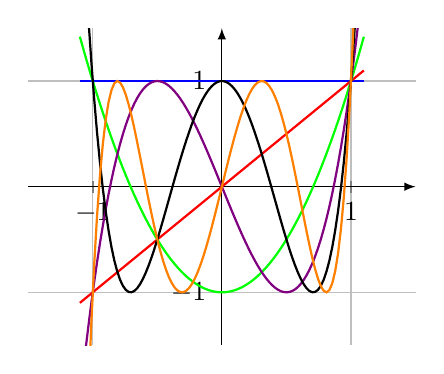
\begin{tikzpicture}
    \begin{axis}[width=6.5cm,
        axis lines=middle,
        inner axis line style={-latex},
        grid=major,
        xmin=-1.5, xmax=1.5,
        ymin=-1.5, ymax=1.5,
        % xlabel=$x$, xlabel style={right},
        % ylabel=$y$, ylabel style={above},
        tick style={thick},
        ticklabel style={font=\normalsize},
        xtick={-1, 0, 1}, 
        ytick={-1, 0, 1},
        % legend entries={0.5x},
            legend style={
            at={(1.05,0.4)},
            anchor=north,
            legend columns=1},
            legend cell align={left}
    ]
    
    \def\a{-1.1}
    \def\b{1.1}
    
    \addplot[blue,thick,samples=100,domain=\a:\b] {1};
    \addplot[red,thick,samples=100,domain=\a:\b] {x};
    \addplot[green,thick,samples=100,domain=\a:\b] {2*x^2-1};
    \addplot[violet,thick,samples=100,domain=\a:\b] {4*x^3-3*x};
    \addplot[black,thick,samples=100,domain=\a:\b] {8*x^4-8*x^2+1};
    \addplot[orange,thick,samples=100,domain=\a:\b] {16*x^5-20*x^3+5*x};
    
   % \legend{$\Leg_0$, 
   %         $\Leg_1$,
%            $\Leg_2$,
%            $\Leg_3$,
 %           $\Leg_4$,
  %          $\Leg_5$
   %         }
    \end{axis}
\end{tikzpicture}
	\caption*{\centering Polynômes de \textsc{Tchebychev} de première espèce}
	\begin{align*}
	   	\color{blue} \Tcheby_0 = 1 \\
    	\color{red} \Tcheby_1 = x \\
    	\color{green} \Tcheby_2 = 2x^2-1 \\
    	\color{purple} \Tcheby_3 = 4x^3-3x \\
    	\color{black} \Tcheby_4 = 8x^4-8x^2+1 \\
    	\color{orange} \Tcheby_5 = 16x^5-20x^3+5x
	\end{align*}
\end{marginfigure}

\begin{preuve}
    \begin{description}
        \item[Existence] Nous allons montrer que la suite $(\Tcheby_n)_{n \geqslant 0}$ vérifie une relation de récurrence. \\
        Soit $n \in \N$,
        \begin{align*}
            \Tcheby_{n+2}(\cos \theta) &= \cos((n+2) \theta) \\
            &= \cos((n+1) \theta) \cos(\theta) - \sin((n+1) \theta) \sin(\theta) \\
            &= \Tcheby_{n+1}(\cos \theta) \cos(\theta) - \frac{1}{2} \left(\cos(n \theta) - \cos((n+2)\theta)\right) \\
            \Tcheby_{n+2}(\cos \theta) &= \Tcheby_{n+1}(\cos \theta) \cos(\theta) - \frac{1}{2} \Tcheby_n(\cos \theta) + \frac{1}{2} \Tcheby_{n+2}(\cos \theta)
        \end{align*}
        d'où
        $$\Tcheby_{n+2} = 2X \Tcheby_{n+1} - \Tcheby_n.$$
        \item[Unicité] L'unicité de $\Tcheby_n$ pour $n$ fixé est garantie pas l'identification de \ptnclegras{deux polynômes coïncidant} sur $]-1, 1[$. 
    \end{description}
\end{preuve}

\marginnote[-6cm]{
    \begin{kaobox}[frametitle=Formule de trigonométrie]
        $$\sin a \sin b = \frac{1}{2} \big( \cos(a-b) - \cos(a+b) \big)$$
    \end{kaobox}
}

\begin{exercice}
    Soit $n \in \N$, déterminer une expression de $\Tcheby_n$.
\end{exercice}  

\begin{solution}
    \begin{align*}
        \cos(n \theta) &= \Reel \left( \me^{\mi n \theta}) = \Reel((\cos \theta + \mi \sin \theta)^n \right)\\
        &= \Reel\left( \sum_{k=0}^n \binom{n}{k} (\cos\theta)^k (\mi \sin\theta)^{n-k} \right) \\
        &= ...
    \end{align*}
    $$\forall n \in \N,\ \Tcheby_n = \sum_{k=0}^{\lfloor n / 2 \rfloor} (-1)^k \binom{n}{2k} X^{n-2k} (1-X^2)^k.$$
\end{solution}

\begin{prop}{}
    \begin{enumerate}
        \item $$\deg \Tcheby_n = n \text{ et } \mathrm{cd}\, \Tcheby_n = 2^{n-1}$$
        \item $\Tcheby_n$ est pair si $n$ est pair et vice versa. \\
        \item Pour tout $n, m$, $\Tcheby_n \circ \Tcheby_m = \Tcheby_{nm}$. \\
        \item $$(1-x^2) \Tcheby''_n(x) - x \Tcheby'_n(x) + n^2 \Tcheby_n(x) = 0.$$
        \item $\Tcheby_n$ admet $n$ racines simples qui sont
        $$a_{k,n} = \cos \left( \frac{(2k-1) \pi}{2n}\right),\ k \in \llbracket 1, n \rrbracket.$$
        \item Sur $[-1, 1]$, $\Tcheby_n$ admet $n+1$ extrema égaux à $1$ en les points
        $$b_{k,n} = \cos\left( \frac{k \pi}{n} \right),\ k \in \llbracket 0, n \rrbracket.$$
    \end{enumerate}
\end{prop}

\begin{preuve}
    \begin{enumerate}
        \item ff
        \item ff
        \item 
    \end{enumerate}
\end{preuve}



\section{Polynômes scindés} \labsec{polynomes_scindes}
\begin{exercice}
    \marginnote[0cm]{Source : \cite{exos_oraux} p. 23}
    Soient $Q \in \R[X]$ et $a \in \R$. On suppose que $Q$ est scindé sur $\R[X]$, montrer que $Q'+aQ$ l'est aussi. 
\end{exercice}

\begin{elem_sol}
    Si $a=0$, appliquer le \ptnclegras{théorème de \textsc{Rolle}} sur chacun des intervalles $[x_i, x_{i+1}]$ où $x_i$ et $x_{i+1}$ sont deux racines réelles consécutives de $Q$.
    \begin{enumerate} 
        \item Poser $\varphi:t \mapsto \exp(at)Q(t)$.
        \item Démarche à revoir.
    \end{enumerate}
\end{elem_sol}

\section{Équation polynomiale} \labsec{equation_polynomiale} \labsec{equation_polynomiale}
\begin{exercice}
    \marginnote[0cm]{Source : \cite{exos_oraux} p. 20}
    Déterminer les polynômes $P \in \C[X]$ tels que:
    $$P\big(X^2\big) = P(X) P(X-1).$$
\end{exercice}
